% ****** Start of file apssamp.tex ******
%
%   This file is part of the APS files in the REVTeX 4.2 distribution.
%   Version 4.2a of REVTeX, December 2014
%
%   Copyright (c) 2014 The American Physical Society.
%
%   See the REVTeX 4 README file for restrictions and more information.
%
% TeX'ing this file requires that you have AMS-LaTeX 2.0 installed
% as well as the rest of the prerequisites for REVTeX 4.2
%
% See the REVTeX 4 README file
% It also requires running BibTeX. The commands are as follows:
%
%  1)  latex apssamp.tex
%  2)  bibtex apssamp
%  3)  latex apssamp.tex
%  4)  latex apssamp.tex
%
\documentclass[%
 reprint,
superscriptaddress,
%groupedaddress,
%unsortedaddress,
%runinaddress,
%frontmatterverbose, 
%preprint,
%preprintnumbers,
%nofootinbib,
%nobibnotes,
%bibnotes,
 amsmath,amssymb,
 aps,13pt
%pra,
%prb,
%rmp,
%prstab,
%prstper,
%floatfix,
]{revtex4-2}
% \usepackage{fontspec}
% \setmainfont{TeX Gyre Termes}
\usepackage{mathtools}
\usepackage{graphicx}% Include figure files
\usepackage{hyperref}
\usepackage{dcolumn}% Align table columns on decimal point
\usepackage{bm}% bold math
%\usepackage{hyperref}% add hypertext capabilities
%\usepackage[mathlines]{lineno}% Enable numbering of text and display math
%\linenumbers\relax % Commence numbering lines

%\usepackage[showframe,%Uncomment any one of the following lines to test 
%%scale=0.7, marginratio={1:1, 2:3}, ignoreall,% default settings
%%text={7in,10in},centering,
%%margin=1.5in,
%%total={6.5in,8.75in}, top=1.2in, left=0.9in, includefoot,
%%height=10in,a5paper,hmargin={3cm,0.8in},
%]{geometry}

% \usepackage[a4paper]{geometry}

\begin{document}
\newcommand{\pos}{\text{pos}}
\newcommand{\sgn}{\text{sgn}}
\preprint{APS/123-QED}

\title{Spider code for single-mode bosonic quantum error detection}% Force line breaks with \\
% \thanks{A footnote to the article title}%

\author{Tien D. Nguyen}
% \altaffiliation[Also at ]{Physics Department, XYZ University.}%Lines break automatically or can be forced with \\
% \author{Second Author}%
%  \email{Second.Author@institution.edu}
\affiliation{%
 Centre for Quantum Technologies, National University of Singapore 117543, Singapore
}%
\affiliation{%
 Faculty of Physics, Hanoi University of Science, VNU Hanoi 120401, Vietnam
}%
% \collaboration{MUSO Collaboration}%\noaffiliation

% \author{Charlie Author}
%  \homepage{http://www.Second.institution.edu/~Charlie.Author}
% \affiliation{
%  Second institution and/or address\\
%  This line break forced% with \\
% }%
% \affiliation{
%  Third institution, the second for Charlie Author
% }%
% \author{Delta Author}
% \affiliation{%
%  Authors' institution and/or address\\
%  This line break forced with \textbackslash\textbackslash
% }%

% \collaboration{CLEO Collaboration}%\noaffiliation

\date{\today}% It is always \today, today,
             %  but any date may be explicitly specified

\begin{abstract}
This paper concerns the construction of a small family of bosonic quantum error-correcting code for single bosonic modes from a fiducial state based on an odd-rotational symmetric state, called the \textsc{spider} state $|S_K\rangle$. The code, invariant under $2\pi/K$ rotations, belongs to a broader family of bosonic codes based on phase-space rotation symmetries. A closed-form expression for the primitive state of the code in the phase-space picture is obtained. Several key differences between the \textsc{spider} code and other types of rotation-symmetric codes are highlighted. Next, the Knill-Laflamme primer matrix is computed for a given set of bosonic errors, including the back-action from measurement and photon loss errors up to order of $K-1$. Finally, a brief discussion on why the code seems to be irredeemable is presented. 
\end{abstract}

%\keywords{Suggested keywords}%Use showkeys class option if keyword
                              %display desired
\maketitle

%\tableofcontents
\section{Introduction}
Continuous-variable quantum information processing using bosonic modes offers a promising alternative to realize robust quantum computation besides using two-level systems as qubits \cite{Joshi_2021, PhysRevA.56.1114}. In the context of quantum error correction, this means bosonic error-correcting schemes with high encoding rates $k/n$, which is the ratio between logical qubits to physical qubits, can be reliably achieved without incurring significant hardware overhead, as compared to their discrete counterparts. This hinges on the fact that redundancies required for quantum information encoding can be naturally introduced by making use of the infinite Hilbert space of only one bosonic mode. It has also been argued that recovery maps for bosonic codes require lower fault-tolerance threshold and less ancillary qubits involved \cite{gkp, gkp_perspective}. From an experimental perspective, realizing high-$Q$ factor, well-controlled bosonic systems is well within reach of current technology; such platforms include superconducting coupled cavities \cite{PhysRevX.13.021004} and motional states of trapped ions \cite{PhysRevLett.124.170502}.

Bosonic error correction codes are broadly characterized into two categories based on their intrinsic symmetry protection. On one end one has codes with discrete translation symmetry, most notably the Gottesman-Kitaev-Preskill (GKP) \cite{gkp} code whose logical codewords are eigenstates of the position and momentum shift operators, protecting the information from small thermal shift in the phase space. One the other end are the family of codes that admits discrete rotation symmetry, namely the cat code \cite{Mirrahimi_2014}, binomial code \cite{bin}, and number-phase code \cite{rotation_symmetric}, which are designed to specifically combat photon loss/gain and dephasing errors. Remarkably enough, GKP codes have been shown numerically to outperform these rotation-symmetric codes under bosonic pure-loss channels at specific small loss rates \cite{performance_structure}. This can be understood by considering an additional phase-insensitive amplification process, which tranforms loss errors to thermal fluctuation noises. It was the cat code, however, that has first gone beyond the error correction break-even point by experimentally demonstrating coherence gain of one fully stabilized, error-corrected logical qubit encoded in a superconducting 3D cavity \cite{devoret, ofek16}.

In this work, I describe a new class of bosonic rotation-symmetric code constructed from a fiducial state called the \textsc{spider} state $|S_K\rangle$ and make comparisions with other types of bosonic codes. Using the Fock-space codeword coefficients \cite{lin22}, I obtain a closed-form expression for the \textsc{Spider} primitive state in the phase-space. The code, by construction, detects $K-1$ photon loss events and is shown to be equipped with a clear protocol to characterize the state preparation of itself. Next, I show that the Knill-Laflamme condition is violated (which is very unfortunate) given a very simple set of bosonic errors. Finally, I discuss how naive renormalization of the Fock-grid coefficients in order to satisfy the QEC primer does not work. 
\section{Bosonic rotation-symmetric codes}
The general task of quantum error correction is to define (or construct) a subspace $C$ of the Hilbert space in which a logical codeword $\rho_L$ is supported that given a set of possible errors $\mathcal{E}$, the measurement of a set of commuting observables results in an error syndrome that can be used to construct a class of completely positive trace-preserving maps $\mathcal{R}$ such that
\begin{align}
    \forall \rho_L \in C: (\mathcal{R}\circ \mathcal{E})(\rho_L) \propto \rho_L. 
\end{align}
While it is true that one can choose any two-dimensional subspace $C$ to formally define a code: simply pick a rank-$2$ projector $P=|0_L\rangle\langle 0_L|+|1_L\rangle\langle 1_L|$ and an associated subspace is defined thereupon, only subspaces having their corresponding error spaces (spanned by $\mathcal{E}(\rho_L)$) being orthogonal \textit{and} undeformed spaces are suitable for error detection \textit{and} correction. Oftentimes, this is too much to ask for: some codes are simply perfect for one type of error, but failed to correct others. This is where \textit{concatenation} comes to rescue. The Shor's code $[[9, 1, 3]]$ \cite{nielsen_chuang_2010}, for example, is constructed by concatenating three-qubit bit flip and phase flip codes, allowing protection against any combination of Pauli $X$ and $Z$ errors on any of the $9$ physical qubits.

Bosonic error-correcting codes share the same set of core principles, with arguably a much more simple model of error processes. The canonical model of bosonic system, the harmonic oscillator for instance, mostly subjects to photon loss errors $\hat{a}$ and dephasing errors $\hat{a}^\dagger \hat{a}$. Photon gain errors $\hat{a}^\dagger$ are also possible, for example, in the cQED architecture where the bosonic mode is dispersively coupled with an anharmonic oscillator (e.g. a 2D transmon qubit) for generation of superposition of photon-number Fock states. In this scenario, energy leakage to the cavity from the ancillary transmon could take place through the Jaynes-Cummings interaction between them. The dominant and most deleterious process is, however, the photon loss errors. Most bosonic codes to this date are designed for detection and correction of cavity photon loss errors. To illustrate this idea, let us consider the simplest case of a bosonic code--the `kitten' code. The logical codewords are even photon-number Fock states,
\begin{align}
    |0_L\rangle = \dfrac{1}{\sqrt{2}}\left(|0\rangle + |4\rangle\right),\quad |1_L\rangle = |2\rangle.
\end{align}
A single loss event maps an arbitrary logical codeword $|\psi_L\rangle = a|0_L\rangle + b|1_L\rangle$ to an odd photon-number state $|\psi_E\rangle =\sqrt{2}(a|3\rangle+b|1\rangle)$. This event can be detected by measuring the photon-number parity $\hat{\Pi}=(-1)^{\hat{n}}$, since $\hat{\Pi}$ admits these states to be $\pm 1$ eigenstates. In other words, the code space and error space are clearly disjoint. More importantly, the information stored in the superposition complex-valued amplitudes $a$ and $b$ is not distorted, permitting the existence of a recovery operator such that it maps the error state ${\hat{a}|\psi_L\rangle}/{\sqrt{\langle\psi_L|\hat{a}^\dagger\hat{a}|\psi_L\rangle}}$ back to the code space, up to some constant $ |\psi_L'\rangle \propto |\psi_L\rangle$. The `kitten' code is therefore a detectable and correctable bosonic code, under the assumption that the error model comprises solely of $\mathcal{E}=\{\hat{I}, \hat{a}\}$. 

Generalization of the `kitten' code leads to the sub-family of binomial code \cite{bin}, whose Fock state coefficients for the logical codewords involved binomial coefficients. It is the enforced spacing in the Fock space structure that gives rise to the detectability properties. A similar idea can be seen in the case of cat code \cite{Mirrahimi_2014} where the logical codewords are superposition of displaced coherent states. The `four-leg' cat code variant, for example, also has an enforced Fock-spacing structure, with codewords being $|0_L\rangle\propto |4n\rangle$ and $|1_L\rangle \propto |4n+2\rangle$, allowing for detection of one photon loss event. However, it should be clear that enforced Fock-spacing (or we shall see later, rotation symmetry in phase space) does not guarantee non-deformed code space, but the fact that both logical codewords having the same average excitation number does.     

It has been shown recently that both binomial code and cat code asymptotically approach a class of bosonic code called number-phase code \cite{rotation_symmetric}, in some parameter regimes. They may even share the same degree of discrete rotation symmetry (e.g. both the kitten code and four-leg cat code are invariant under $180^\circ$ rotation). Loosely speaking, they only differ from each other in either the amplitude of Fock space coefficients, or the un-rotated \textit{primitive} state in the phase space. This class of bosonic code is called rotation-symmetric codes. In what follows I briefly summarize the overarching framework used to study these codes and highlight a key properties that motivates the construction of the \textsc{spider} code later.
\subsection{Logical codewords}
A subspace is said to have $K$-fold rotation symmetry if any state in the codespace is a $+1$ eigenstate of the discrete rotation operator,
\begin{align}
    \hat{R}_K = \exp\left[i({2\pi}/{K})\hat{n}\right], 
\end{align}
where $\hat{n}=\hat{a}^\dagger\hat{a}$ is the photon-number operator. Using this, we can define a rotation-symmetric code of order $K$ to be a subspace in which the operator $\hat{R}_{2K}$ acts non-trivially as the logical $\bar{Z}$ gate
\begin{align}\label{logical_Z}
    \bar{Z} \coloneqq \hat{R}_K = \exp\left[i({\pi}/{K})\hat{n}\right].
\end{align}
\subsubsection{Fock space structure}
The definition of a bosonic rotation code (\ref{logical_Z}) enforces a Fock-grid spacing structure. Indeed, any logical codeword can be written as $|\psi_L\rangle = \sum_{m}c_m|m\rangle$. Since logical zero/one state must be $\pm 1$ eigenstate of $\bar{Z}$, the logical zero has support on every even $|2mK\rangle$ Fock states and the logical one has support on every odd $|(2m+1)K\rangle$ Fock states
\begin{align}
    |0_K\rangle &= \sum_{m=0}^\infty c_{2mK}|2mK\rangle,\\
    |1_K\rangle &= \sum_{m=0}^\infty c_{(2m+1)K}|(2m+1)K\rangle.
\end{align}
The dual-basis codewords are thus also defined via equal superposition of the computational codewords,
\begin{align}
    |\pm_K\rangle &= \dfrac{1}{\sqrt{2}}\sum_{m=0}^\infty  (\pm 1)^{m}c_{mK} |mK\rangle,
\end{align}
Both logical $|\pm_K\rangle$ states have full support on every $|mK\rangle$ Fock states, with an additional $e^{i\pi}$ phase of the logical minus state on every odd $m$ to ensure orthogonality. This motivates the construction of the new \textsc{spider} code, which will be explored further in later parts.
\subsubsection{Phase space structure}
To complete the description, let us explore the phase space structure of bosonic rotation codes. From the definition ($\ref{logical_Z}$) it can be seen that the logical codewords are discrete rotated superposition of some primitive states $|\Phi\rangle$. The following two states are also $+1$ and $-1$ eigenstates of the logical $\bar{Z}=\exp[i(\pi/K)\hat{n}]$ operator,
\begin{align}
    |0_\Phi\rangle = \dfrac{1}{\sqrt{N}_0}\sum_{m=0}^{2N-1}e^{i(m\pi/K)\hat{n}}|\Phi\rangle,\\
    |1_\Phi\rangle = \dfrac{1}{\sqrt{N}_1}\sum_{m=0}^{2N-1}(-1)^me^{i(m\pi/K)\hat{n}}|\Phi\rangle,
\end{align}
where $N_i$ are the normalization constants. To bridge the two presentations, we use the Kronecker's comb $\frac{1}{K}\sum_{m=0}^{K-1}e^{i(2\pi mn/K)}=\sum_{k=0}^{\infty}\delta_{n,mK}$ to construct a projector onto the subspace spanned by $\{|2mK+\ell\rangle\}$ Fock states,
\begin{align}
    \hat{\Pi}^{\ell}_{2K} &\coloneqq \sum_{m=0}^\infty |2mK+\ell\rangle\langle 2mK+\ell|\\
    &=\dfrac{1}{2K}\sum_{k=0}^{2K-1}\left(e^{-i(\pi\ell/K)}e^{i(\pi/K)\hat{n}}\right)^m
\end{align}
Now, given a primitive state $|\Phi\rangle=\sum_n c_n|n\rangle$, it can be seen that the projection of this state onto $\{|2mK+\ell\rangle\}$ is simply
\begin{align}
    \hat{\Pi}^{\ell}_{2K}|\Phi\rangle \propto \sum_{m=0}^\infty c_{2mK+\ell}|2mK+\ell\rangle,
\end{align}
which is a $e^{i\pi\ell/K}$ eigenstate of the logical $\bar{Z}$ operator. Upon specifying $\ell=0$ or $\ell=K$, one re-obtains the logical zero and one with support on even/odd Fock states, as mentioned above.
\begin{figure*}
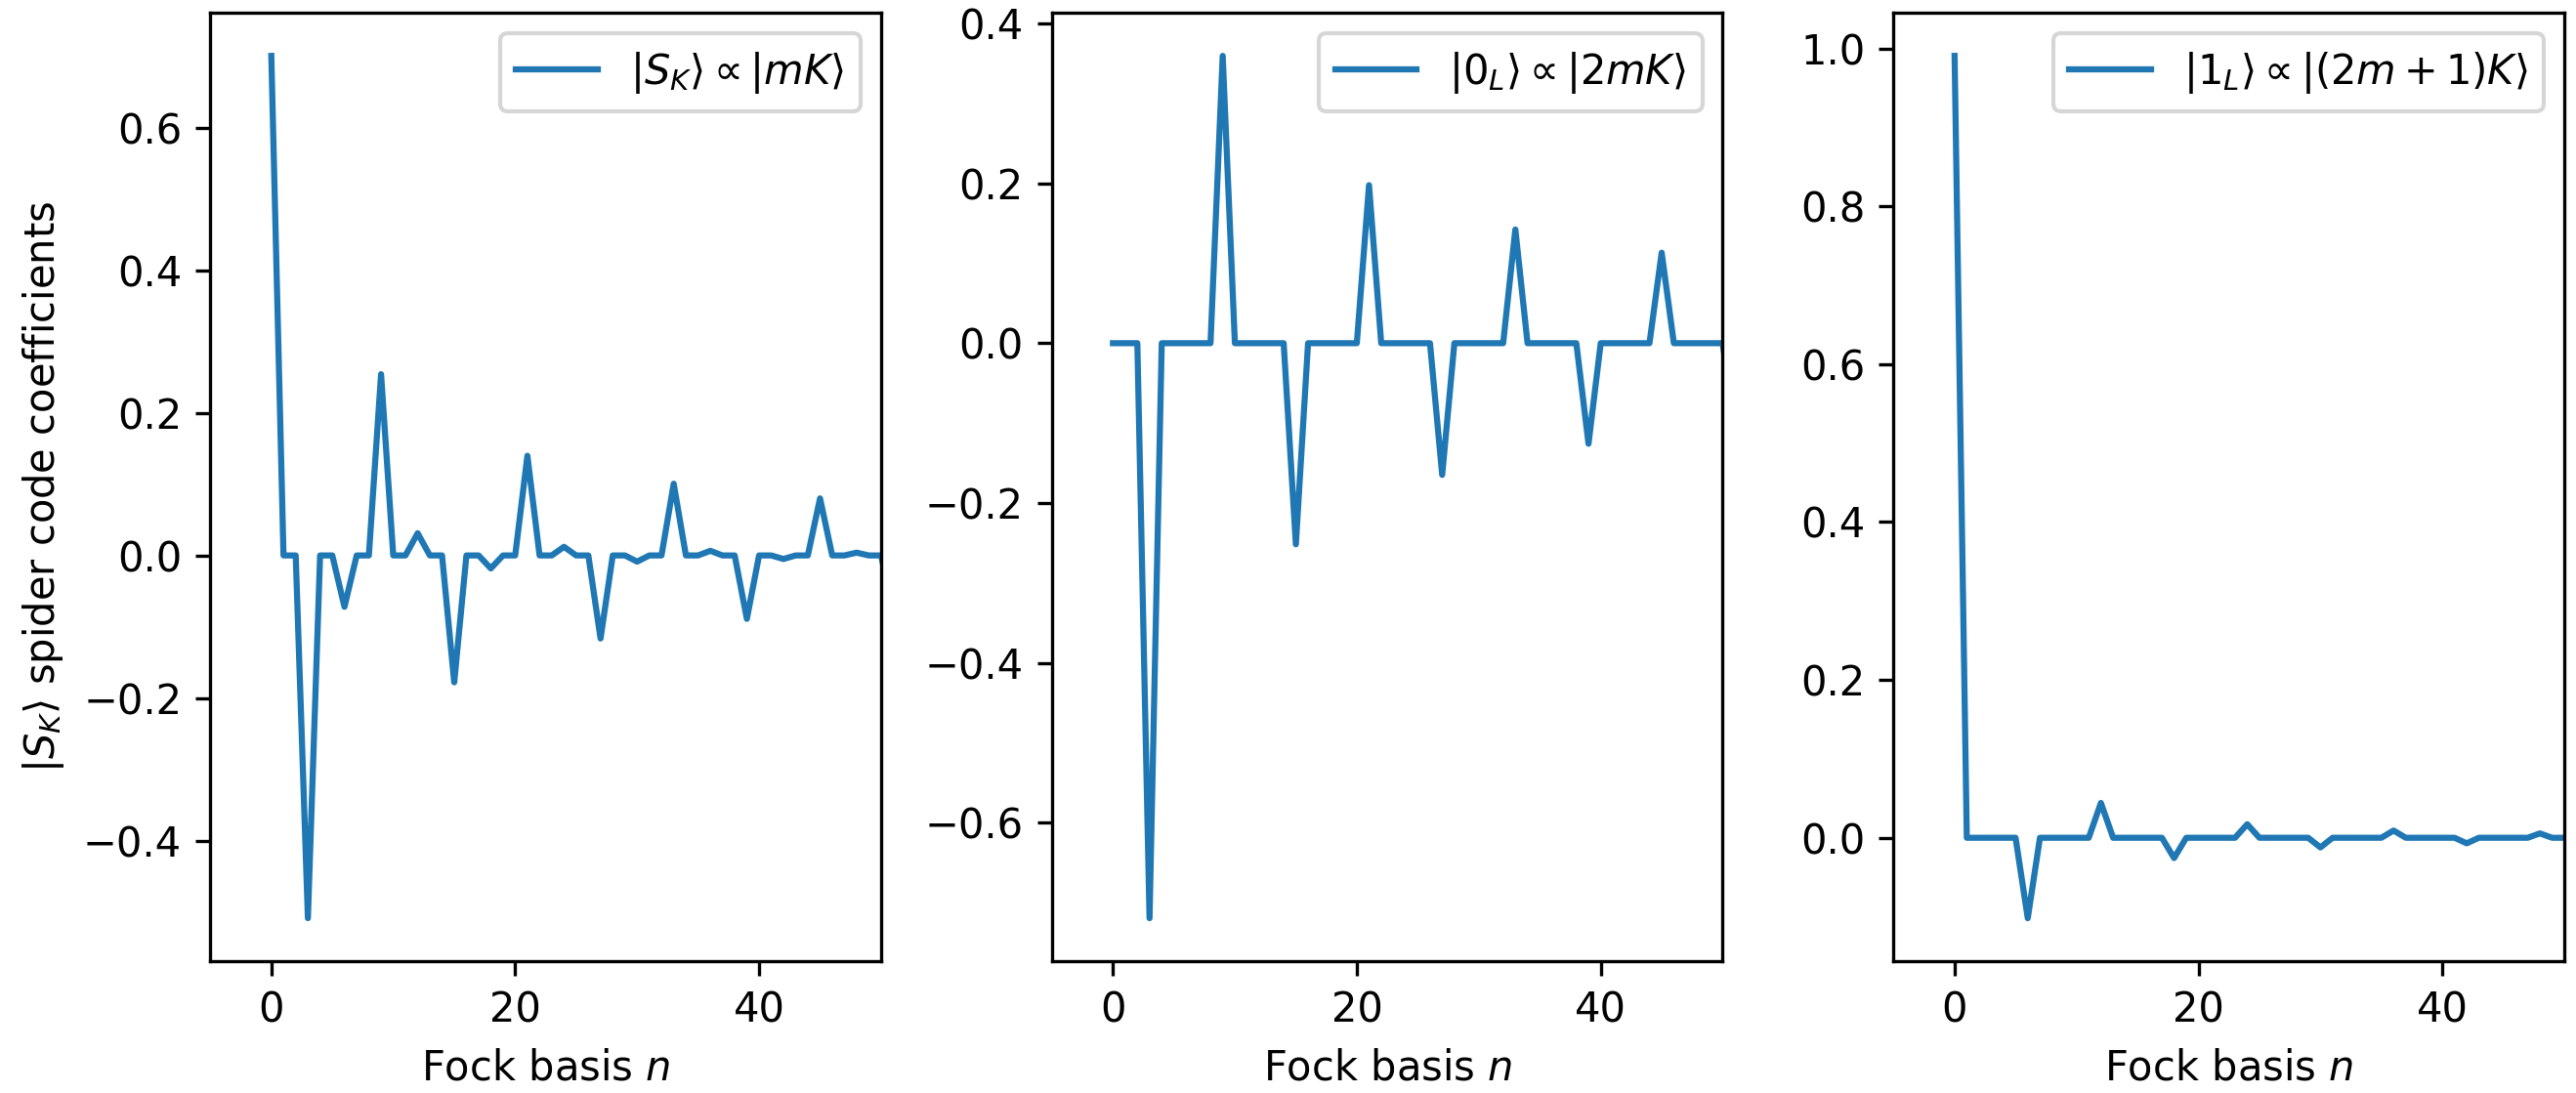
\includegraphics[scale=0.75]{ss_coeffs.png}% Here is how to import EPS art
\caption{\label{fig:ss_coeffs}The \textsc{spider} state (a) is of the form $\sum_m(-1)^{\lceil m/2 \rceil}s_{mK}|mK\rangle$ where $s_{mK}\in \mathbb{R}$. The coefficients are found numerically with truncation at $n=5000$ Fock states. (b) and (c) The corresponding logical codewords defined from the \textsc{spider} state.}
\end{figure*}
\subsection{Encoded logical operators}
The construction of rotation-symmetric codes implies the natural existence of the encoded logical $\bar{Z}$ operator. The encoded logical $\bar{X}$ operator is however more subtle. One can write something as simple as the number-translation operator
\begin{align}
    \bar{X}_K \coloneqq \sum_{n}^\infty |n\rangle\langle n + K|,
\end{align}
that will map states with support on odd to even Fock states, and vice versa. But $\bar{X}_K$ is non-unitary. The coefficients are also required to be \textit{exactly} the same. This is the case of the number-phase codes, whose codewords are Pegg-Barnett phase states and not normalizable. Because the Fock state amplitudes are the same, the code implies a vanishing phase uncertainty limit, and to some extent, non-physicality. Number-phase code admits the $\bar{X}_K$ and $\bar{X}_{2K}$ to be its logical $\bar{X}$ operator and stabilizer operator, respectively. 
\subsection{Code distance}
In the stabilizer formalism for two-level qubit codes, the code distance is defined as the minimum weight of the set of encoded logical operators. The intuition for this definition comes from the fact that for a $k$-distance code, it takes an error exactly $k$ steps to get from one codeword to another, making such error undetected.

Bosonic rotation-symmetric codes have the same notion of code distance. In fact, there are two equivalent representations, hence two notions of code distance, namely \textit{number distance} and \textit{rotational distance}. More specifically, a code that is $K$-fold rotation symmetric will have number distance $d_n = K$ and rotational distance $d_\theta=\pi/K$. In words, increased spacing in Fock space allows for detection of more loss events: a number-shift error smaller than $k$ will be guaranteed detected by a rotation-symmetric code with $K$-fold symmetry where $K>k$. Similarly, errors that lead to small angle rotations $\theta < d_\theta$ in phase space picture will also be detectable by an order-$K$ code. 
\subsection{Finding new rotation codes?}
The structure of a rotation-symmetric code requires nothing but a subspace with $K$-fold discrete symmetry. The choice of coefficient amplitudes or the primitive states rather reflects the exact experimental implementation. In realistic parameter regime, where it requires less than 5 photons stored in the cavity, both cat code (at sweet-spot values), and binomial code follow approximately the same distribution in the Fock space, resulting in similar performance under the same pure loss channel \cite{performance_structure, rotation_symmetric}.

A bosonic code that inherits $K$-fold symmetry while came equipped with a nice protocol for characterization is therefore of interest. Next, I describe how to find such a code, called the \textsc{spider} code.
\section{The spider code}
\begin{figure}[]
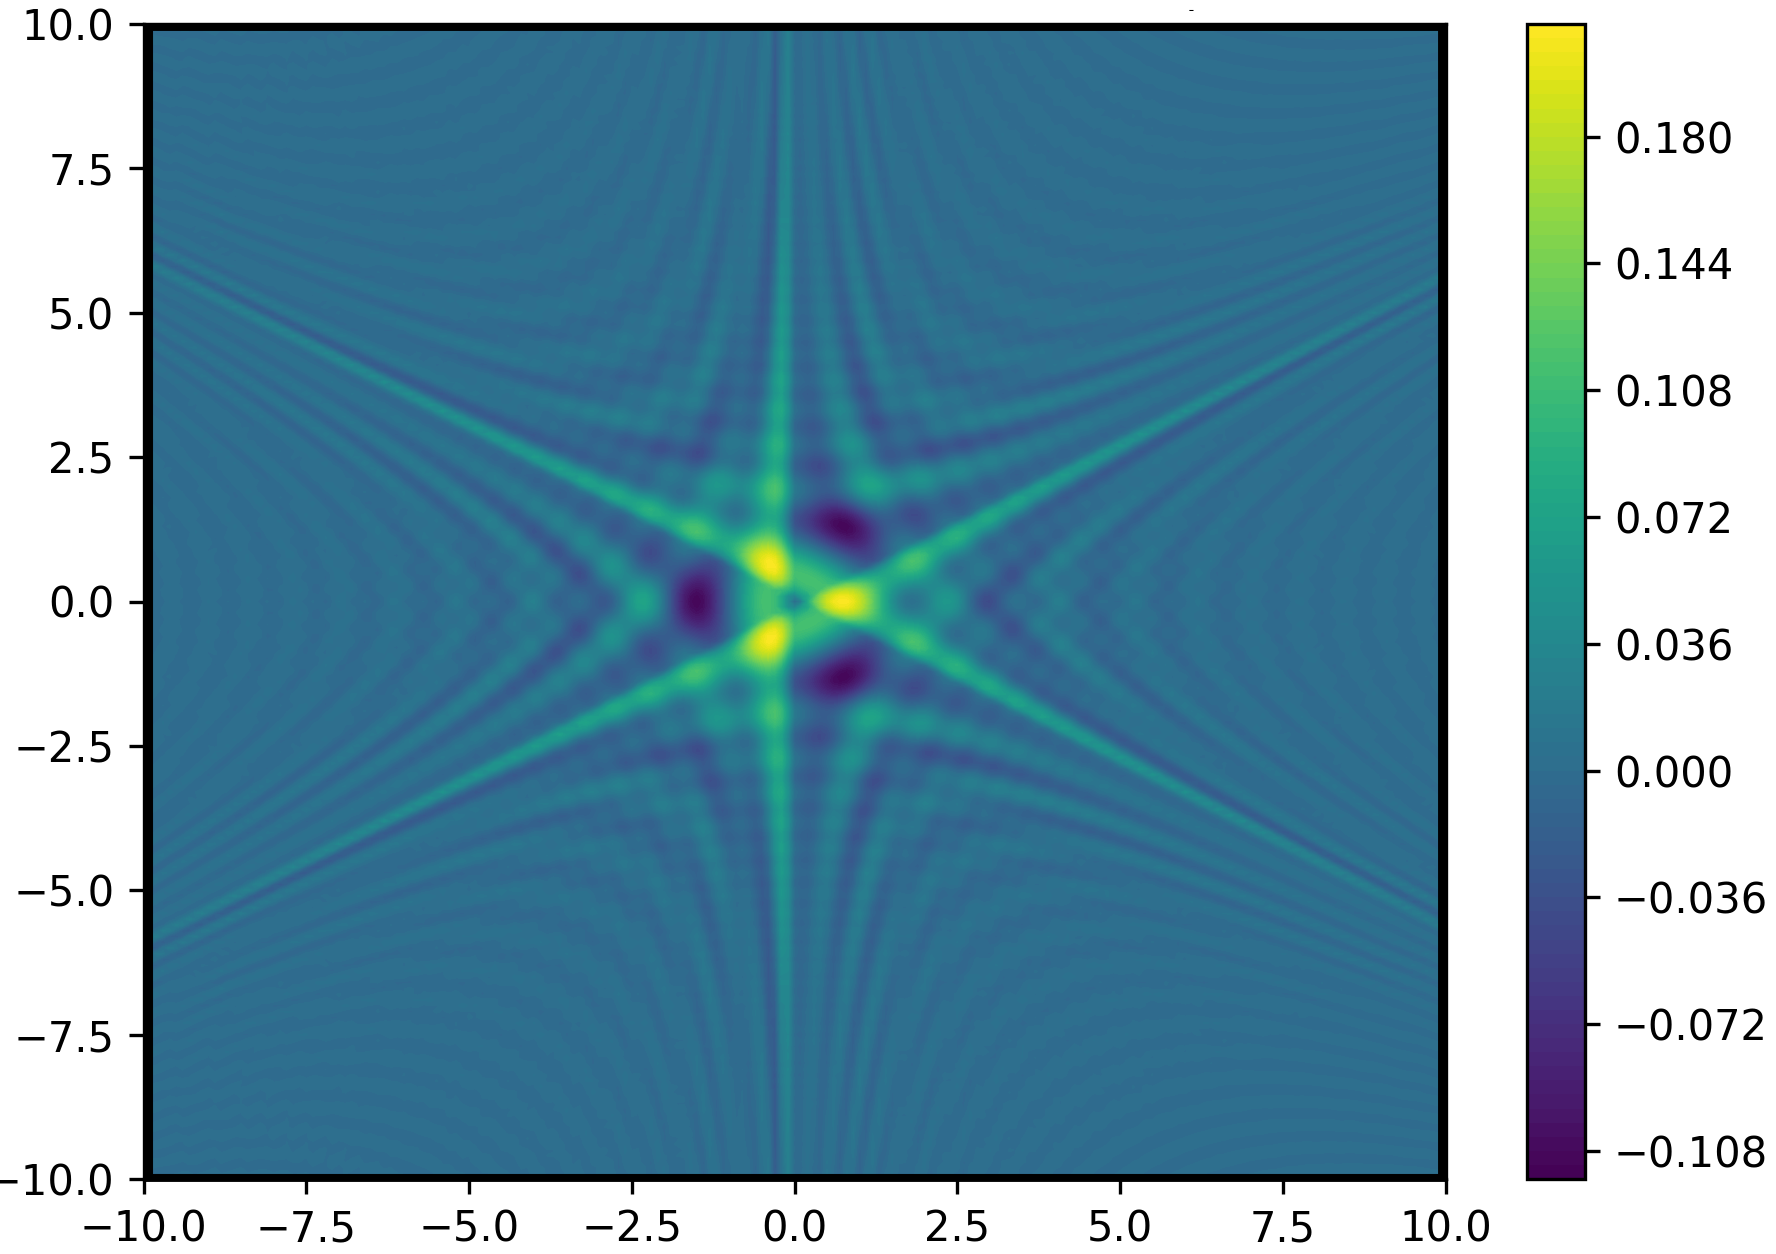
\includegraphics[scale=0.55]{wigerK=3.png}% Here is how to import EPS art
\caption{\label{fig:wigner3} Wigner function $W(x,p)$ of the \textsc{spider} state that maximally violates the classical bound for $K=3$.}
\end{figure}
It all starts with the so-called \textsc{spider} state $|S_K\rangle$. The \textsc{spider} state has support on the full set of $|mK\rangle$ Fock states, i.e. it defines a subspace with $K$-fold symmetry, therefore coincides with the definition of the logical plus state $|+_K\rangle$, and unambiguously defines the rank-2 projector needed to define the codespace,
\begin{align}
    \hat{P} = |0_K\rangle\langle 0_K\rangle + |1_K\rangle\langle 1_K|,
\end{align}
where the logical codewords are defined upon the fiducial \textsc{spider} state $|S_K\rangle$,
\begin{align}
    |S_K\rangle \coloneqq |+_K\rangle = \sum_{m=0}^{\infty} s_{mK}|mK\rangle = \dfrac{|0_K\rangle + |1_K\rangle}{\sqrt{2}}.
\end{align}
The \textsc{spider} states, specified by an order-$K$ symmetry, is special in the sense that they maximally violate the so-called classicality feature of a quantum harmonic oscillator in uniform precessions \cite{lin22}\cite{tsirelson2006coordinate}.
\subsection{Precession protocol}
Here I revisit the general criterion to find such states. As it is often the case in physics, we consider a harmonic oscillator, whose dynamics generated by the time-indepedent Hamiltonian $H(x,p)=p^2/2m+m\omega_0^2x^2/2$. The canonical variables $x(t)$ and $p(t)$ undergo a uniform precession in the phase space with period $T_0=2\pi/\omega_0$. To faithfully verify whether the harmonic oscillator is a quantum object, or a classical object, one can perform a nonclassicality check protocol \cite{lin22}. In short, after repeatedly prepare the state of the system (in an arbitrary manner), the sign of $x$ (or $p$) is measured at one of $K$ different instances given by $t_k=(k/K)/T$, where $K>0$ and $T=T_0$. After several rounds, the probability that the sign of $x$ is positive is estimated by
\begin{align}
    P_K = \dfrac{1}{K}\sum_{k=0}^{K-1}\left(\text{Pr}[A_1(t_k)>0]+\dfrac{1}{2}\text{Pr}[A_1(t_k=0)]\right).
\end{align}
A classical harmonic oscillator $\mathbf{P}^c_K$ score will be $1/2$ for $K$ even, and bounded above by
\begin{align}
    \mathbf{P}^c_K=\dfrac{1}{2}\left(1+\dfrac{1}{K}\right)\quad\text{for $K$ odd}.
\end{align}
The crucial observation is that, a quantum harmonic oscillator undergoing the same dynamics generated by $H(x,p)$ will have the score $\mathbf{P}^\infty_K>\mathbf{P}^c_K$, where $\mathbf{P}^\infty_K=\text{tr}(\rho \hat{Q}_K)$ and
\begin{align}
    \hat{Q}_K = \dfrac{1}{K}\sum_0^{K-1}\text{pos}[X(t_k)],
\end{align}
with $\text{pos}(X)$ defined such that $\text{pos}(X)=1/2[1+\text{sgn(X)}]$. The maximum quantum score is obtained when $\rho=|S_K\rangle\langle S_K|$, which is the eigenstate of $\hat{Q}_K$ with the largest eigenvalue. For $K=3$, the quantum score is as large as $\mathbf{P}^\infty_3 \gtrsim 0.709 > \mathbf{P}_3^c=2/3$. This gap can be attributed to the fact that $\rho$ corresponds to a non-classical probability distribution with suitable negativity presences. The state $|S_K\rangle$ is the mentioned \textsc{spider} state, with support on every $|mK\rangle$ Fock states. The Wigner's function $W(x,p)$ of the \textsc{spider} state (Fig. \ref{fig:wigner3}) clearly demonstrates the idea of concentrated negativities.
\subsection{Construction fidelity}
In additional to an intrinsic gap between quantum and classical scores, $\vert\vert P^\infty_K-P^c_K\vert\vert$, the eigen-spectrum of $\hat{Q}_K$ itself implies an $\epsilon$ gap between the largest and second largest eigenvalues, let them be $q_d$ and $q_{d-1}$ for convenience purpose. 
\begin{align}
    q_d - q_{d-1} > \epsilon.
\end{align}
The observation is that, an arbitrary realization of $|S_K\rangle$ will always be verifiable. More importantly, it can be proved that the distance between an arbitrary mixed state and the \textsc{spider} state $|S_K\rangle$ is bounded below. This is the crucial element enabling faithful verification of the \textsc{spider} state.

Let us suppose the arbitrary mixed state $\rho=\sum_{j=1}^N p_j|\phi_j\rangle\langle\phi_j|$. The `distance' between $\rho$ and $\rho_K$ is
\begin{align}
    F &= \langle S_K|\left(\sum_{j=1}^N p_j|\phi_j\rangle\langle\phi_j|\right)|S_K\rangle\\
    &= \sum_{j=1}^N p_j \langle\phi_j|S_K\rangle\langle S_K |\phi_j\rangle\label{twenty-one}
\end{align}
Using the spectral theorem,
\begin{align}
    \hat{Q}_K=\sum_{k=1}^{d-1}q_k|q_k\rangle\langle q_k|+q_d|S_K\rangle\langle S_K|
\end{align}
Substituting to (\ref{twenty-one}),
\begin{align}
    F &= \dfrac{1}{q_d}\sum_{j=1}^N p_j \langle\phi_j|\left(\hat{Q}_K-\sum_{k=1}^{d-1}q_k|q_k\rangle\langle q_k|\right)|\phi_j\rangle\\
    &=\dfrac{1}{q_d}\sum_{j=1}^N p_j \langle\phi_j|\hat{Q}_K|\phi_j\rangle -\sum_{j=1}^{N}\sum_{k=1}^{d-1}\dfrac{p_j q_k}{q_d}\langle\phi_j|q_k\rangle\langle q_k|\phi_j\rangle
\end{align}
where
\begin{align}
    \sum_{j}p_j\langle \phi_j|\hat{Q}_K|\phi_j\rangle=\sum_{k=1} q_k \text{Tr}\left(\rho |q_k\rangle \langle q_k|\right)
\end{align} 
is the expectation value conditioned on the state $\rho$. This weighted sum is special since the dominant eigenvalue of $\hat{Q}_K$ is $q_d$, this means given an arbitrary probability distribution, $\langle \hat{Q}_K\rangle = q_d-\epsilon > q_{d-1}$. Hence 
\begin{align}
    F = 1 - \dfrac{\epsilon}{q_d} - A
\end{align}
Let us now consider the lower bound and upper bound of $A$. First, the upper bound
\begin{align}
\max A &\leq \max \sum_{j=1}^N\sum_{k=1}^{d-1} p_j\dfrac{q_{d-1}}{q_d} |\langle\phi_j|q_k\rangle|^2\\
&= \dfrac{q_{d-1}}{q_d}\max \sum_{j=1}^N p_j \sum_{k=1}^{d-1} |\langle\phi_j|q_k\rangle|^2\\
&= \dfrac{q_{d-1}}{q_d}
\end{align}
Similar trick for the lower bound,
\begin{align}
\max A \geq \sum_{j=1}^N\sum_{k=1}^{d-1} p_j \dfrac{q_k}{q_d} |\langle\tilde{\phi}_j|q_k\rangle|^2
\end{align}
where $\tilde{\phi}_j$ is an arbitrary state we can construct. The question is, can we construct a state that pushes
\begin{align}
    \sum_{j=1}^N\sum_{k=1}^{d-1} p_j \dfrac{q_k}{q_d} |\langle\tilde{\phi}_j|q_k\rangle|^2
\end{align}
up as high as possible? Yes, let $\tilde{\phi}_1=q_{d-1}$ and at the same time $p_1=1\ (p_2=p_3=\dots=p_N=0)$, so that
\begin{align}
\max A &\geq \sum_{j=1}^N\sum_{k=1}^{d-1} p_j \dfrac{q_k}{q_d} |\langle\tilde{\phi}_j|q_k\rangle|^2\\
&= \dfrac{q_{d-1}}{q_d} 
\end{align}
Hence $\max A = {q_{d-1}}/{q_d}$ (an arbitrary mixed state $\rho$). In conclusion, the minimum distance between $|q_d\rangle$ and a mixed state $\rho$ can only be as low as
\begin{align}
F = 1-\dfrac{\epsilon+q_{d-1}}{q_d} > 0,
\end{align}
making the \textsc{spider} never mislabelled with an arbitrary mixed state. 
\subsection{Comparisons with other codes}
\subsubsection{Average excitation number}
To compare the size of bosonic codes, one can look at the average excitation number,
\begin{align}
    \bar{n}_{\text{code}} = \text{tr}[\hat{P}_{\text{code}}\hat{n}]/2,
\end{align}
where $\hat{P}$ is the rank-2 projector onto the codespace. This number is proportional to the average energy required to construct a code state. While the average excitation number is the same for each of the dual-basis codewords $|\pm_K\rangle$, it can be different for the computational codewords. This is the Achilles' heel of the \textsc{spider} code, preventing the code from being error-correctable.
% \section{\label{sec:level1}First-level heading:\protect\\ The line
% break was forced \lowercase{via} \textbackslash\textbackslash}

% This sample document demonstrates proper use of REV\TeX~4.2 (and
% \LaTeXe) in mansucripts prepared for submission to APS
% journals. Further information can be found in the REV\TeX~4.2
% documentation included in the distribution or available at
% \url{http://journals.aps.org/revtex/}.

% When commands are referred to in this example file, they are always
% shown with their required arguments, using normal \TeX{} format. In
% this format, \verb+#1+, \verb+#2+, etc. stand for required
% author-supplied arguments to commands. For example, in
% \verb+\section{#1}+ the \verb+#1+ stands for the title text of the
% author's section heading, and in \verb+\title{#1}+ the \verb+#1+
% stands for the title text of the paper.

% Line breaks in section headings at all levels can be introduced using
% \textbackslash\textbackslash. A blank input line tells \TeX\ that the
% paragraph has ended. Note that top-level section headings are
% automatically uppercased. If a specific letter or word should appear in
% lowercase instead, you must escape it using \verb+\lowercase{#1}+ as
% in the word ``via'' above.

% \subsection{\label{sec:level2}Second-level heading: Formatting}

% This file may be formatted in either the \texttt{preprint} or
% \texttt{reprint} style. \texttt{reprint} format mimics final journal output. 
% Either format may be used for submission purposes. \texttt{letter} sized paper should
% be used when submitting to APS journals.

% \subsubsection{Wide text (A level-3 head)}
% The \texttt{widetext} environment will make the text the width of the
% full page, as on page~\pageref{eq:wideeq}. (Note the use the
% \verb+\pageref{#1}+ command to refer to the page number.) 
% \paragraph{Note (Fourth-level head is run in)}
% The width-changing commands only take effect in two-column formatting. 
% There is no effect if text is in a single column.

% \subsection{\label{sec:citeref}Citations and References}
% A citation in text uses the command \verb+\cite{#1}+ or
% \verb+\onlinecite{#1}+ and refers to an entry in the bibliography. 
% An entry in the bibliography is a reference to another document.

% \subsubsection{Citations}
% Because REV\TeX\ uses the \verb+natbib+ package of Patrick Daly, 
% the entire repertoire of commands in that package are available for your document;
% see the \verb+natbib+ documentation for further details. Please note that
% REV\TeX\ requires version 8.31a or later of \verb+natbib+.

% \paragraph{Syntax}
% The argument of \verb+\cite+ may be a single \emph{key}, 
% or may consist of a comma-separated list of keys.
% The citation \emph{key} may contain 
% letters, numbers, the dash (-) character, or the period (.) character. 
% New with natbib 8.3 is an extension to the syntax that allows for 
% a star (*) form and two optional arguments on the citation key itself.
% The syntax of the \verb+\cite+ command is thus (informally stated)
% \begin{quotation}\flushleft\leftskip1em
% \verb+\cite+ \verb+{+ \emph{key} \verb+}+, or\\
% \verb+\cite+ \verb+{+ \emph{optarg+key} \verb+}+, or\\
% \verb+\cite+ \verb+{+ \emph{optarg+key} \verb+,+ \emph{optarg+key}\ldots \verb+}+,
% \end{quotation}\noindent
% where \emph{optarg+key} signifies 
% \begin{quotation}\flushleft\leftskip1em
% \emph{key}, or\\
% \texttt{*}\emph{key}, or\\
% \texttt{[}\emph{pre}\texttt{]}\emph{key}, or\\
% \texttt{[}\emph{pre}\texttt{]}\texttt{[}\emph{post}\texttt{]}\emph{key}, or even\\
% \texttt{*}\texttt{[}\emph{pre}\texttt{]}\texttt{[}\emph{post}\texttt{]}\emph{key}.
% \end{quotation}\noindent
% where \emph{pre} and \emph{post} is whatever text you wish to place 
% at the beginning and end, respectively, of the bibliographic reference
% (see Ref.~[\onlinecite{witten2001}] and the two under Ref.~[\onlinecite{feyn54}]).
% (Keep in mind that no automatic space or punctuation is applied.)
% It is highly recommended that you put the entire \emph{pre} or \emph{post} portion 
% within its own set of braces, for example: 
% \verb+\cite+ \verb+{+ \texttt{[} \verb+{+\emph{text}\verb+}+\texttt{]}\emph{key}\verb+}+.
% The extra set of braces will keep \LaTeX\ out of trouble if your \emph{text} contains the comma (,) character.

% The star (*) modifier to the \emph{key} signifies that the reference is to be 
% merged with the previous reference into a single bibliographic entry, 
% a common idiom in APS and AIP articles (see below, Ref.~[\onlinecite{epr}]). 
% When references are merged in this way, they are separated by a semicolon instead of 
% the period (full stop) that would otherwise appear.

% \paragraph{Eliding repeated information}
% When a reference is merged, some of its fields may be elided: for example, 
% when the author matches that of the previous reference, it is omitted. 
% If both author and journal match, both are omitted.
% If the journal matches, but the author does not, the journal is replaced by \emph{ibid.},
% as exemplified by Ref.~[\onlinecite{epr}]. 
% These rules embody common editorial practice in APS and AIP journals and will only
% be in effect if the markup features of the APS and AIP Bib\TeX\ styles is employed.

% \paragraph{The options of the cite command itself}
% Please note that optional arguments to the \emph{key} change the reference in the bibliography, 
% not the citation in the body of the document. 
% For the latter, use the optional arguments of the \verb+\cite+ command itself:
% \verb+\cite+ \texttt{*}\allowbreak
% \texttt{[}\emph{pre-cite}\texttt{]}\allowbreak
% \texttt{[}\emph{post-cite}\texttt{]}\allowbreak
% \verb+{+\emph{key-list}\verb+}+.

% \subsubsection{Example citations}
% By default, citations are numerical\cite{Beutler1994}.
% Author-year citations are used when the journal is RMP. 
% To give a textual citation, use \verb+\onlinecite{#1}+: 
% Refs.~\onlinecite{[][{, and references therein}]witten2001,Bire82}. 
% By default, the \texttt{natbib} package automatically sorts your citations into numerical order and ``compresses'' runs of three or more consecutive numerical citations.
% REV\TeX\ provides the ability to automatically change the punctuation when switching between journal styles that provide citations in square brackets and those that use a superscript style instead. This is done through the \texttt{citeautoscript} option. For instance, the journal style \texttt{prb} automatically invokes this option because \textit{Physical 
% Review B} uses superscript-style citations. The effect is to move the punctuation, which normally comes after a citation in square brackets, to its proper position before the superscript. 
% To illustrate, we cite several together 
% \cite{[See the explanation of time travel in ]feyn54,*[The classical relativistic treatment of ][ is a relative classic]epr,witten2001,Berman1983,Davies1998,Bire82}, 
% and once again in different order (Refs.~\cite{epr,feyn54,Bire82,Berman1983,witten2001,Davies1998}). 
% Note that the citations were both compressed and sorted. Futhermore, running this sample file under the \texttt{prb} option will move the punctuation to the correct place.

% When the \verb+prb+ class option is used, the \verb+\cite{#1}+ command
% displays the reference's number as a superscript rather than in
% square brackets. Note that the location of the \verb+\cite{#1}+
% command should be adjusted for the reference style: the superscript
% references in \verb+prb+ style must appear after punctuation;
% otherwise the reference must appear before any punctuation. This
% sample was written for the regular (non-\texttt{prb}) citation style.
% The command \verb+\onlinecite{#1}+ in the \texttt{prb} style also
% displays the reference on the baseline.

% \subsubsection{References}
% A reference in the bibliography is specified by a \verb+\bibitem{#1}+ command
% with the same argument as the \verb+\cite{#1}+ command.
% \verb+\bibitem{#1}+ commands may be crafted by hand or, preferably,
% generated by Bib\TeX. 
% REV\TeX~4.2 includes Bib\TeX\ style files
% \verb+apsrev4-2.bst+, \verb+apsrmp4-2.bst+ appropriate for
% \textit{Physical Review} and \textit{Reviews of Modern Physics},
% respectively.

% \subsubsection{Example references}
% This sample file employs the \verb+\bibliography+ command, 
% which formats the \texttt{\jobname .bbl} file
% and specifies which bibliographic databases are to be used by Bib\TeX\ 
% (one of these should be by arXiv convention \texttt{\jobname .bib}).
% Running Bib\TeX\ (via \texttt{bibtex \jobname}) 
% after the first pass of \LaTeX\ produces the file
% \texttt{\jobname .bbl} which contains the automatically formatted
% \verb+\bibitem+ commands (including extra markup information via
% \verb+\bibinfo+ and \verb+\bibfield+ commands). 
% If not using Bib\TeX, you will have to create the \verb+thebibiliography+ environment 
% and its \verb+\bibitem+ commands by hand.

% Numerous examples of the use of the APS bibliographic entry types appear in the bibliography of this sample document.
% You can refer to the \texttt{\jobname .bib} file, 
% and compare its information to the formatted bibliography itself.

% \subsection{Footnotes}%
% Footnotes, produced using the \verb+\footnote{#1}+ command, 
% usually integrated into the bibliography alongside the other entries.
% Numerical citation styles do this%
% \footnote{Automatically placing footnotes into the bibliography requires using BibTeX to compile the bibliography.};
% author-year citation styles place the footnote at the bottom of the text column.
% Note: due to the method used to place footnotes in the bibliography, 
% \emph{you must re-run Bib\TeX\ every time you change any of your document's footnotes}. 

% \section{Math and Equations}
% Inline math may be typeset using the \verb+$+ delimiters. Bold math
% symbols may be achieved using the \verb+bm+ package and the
% \verb+\bm{#1}+ command it supplies. For instance, a bold $\alpha$ can
% be typeset as \verb+$\bm{\alpha}$+ giving $\bm{\alpha}$. Fraktur and
% Blackboard (or open face or double struck) characters should be
% typeset using the \verb+\mathfrak{#1}+ and \verb+\mathbb{#1}+ commands
% respectively. Both are supplied by the \texttt{amssymb} package. For
% example, \verb+$\mathbb{R}$+ gives $\mathbb{R}$ and
% \verb+$\mathfrak{G}$+ gives $\mathfrak{G}$

% In \LaTeX\ there are many different ways to display equations, and a
% few preferred ways are noted below. Displayed math will center by
% default. Use the class option \verb+fleqn+ to flush equations left.

% Below we have numbered single-line equations; this is the most common
% type of equation in \textit{Physical Review}:
% \begin{eqnarray}
% \chi_+(p)\alt{\bf [}2|{\bf p}|(|{\bf p}|+p_z){\bf ]}^{-1/2}
% \left(
% \begin{array}{c}
% |{\bf p}|+p_z\\
% px+ip_y
% \end{array}\right)\;,
% \\
% \left\{%
%  \openone234567890abc123\alpha\beta\gamma\delta1234556\alpha\beta
%  \frac{1\sum^{a}_{b}}{A^2}%
% \right\}%
% \label{eq:one}.
% \end{eqnarray}
% Note the open one in Eq.~(\ref{eq:one}).

% Not all numbered equations will fit within a narrow column this
% way. The equation number will move down automatically if it cannot fit
% on the same line with a one-line equation:
% \begin{equation}
% \left\{
%  ab12345678abc123456abcdef\alpha\beta\gamma\delta1234556\alpha\beta
%  \frac{1\sum^{a}_{b}}{A^2}%
% \right\}.
% \end{equation}

% When the \verb+\label{#1}+ command is used [cf. input for
% Eq.~(\ref{eq:one})], the equation can be referred to in text without
% knowing the equation number that \TeX\ will assign to it. Just
% use \verb+\ref{#1}+, where \verb+#1+ is the same name that used in
% the \verb+\label{#1}+ command.

% Unnumbered single-line equations can be typeset
% using the \verb+\[+, \verb+\]+ format:
% \[g^+g^+ \rightarrow g^+g^+g^+g^+ \dots ~,~~q^+q^+\rightarrow
% q^+g^+g^+ \dots ~. \]


% \subsection{Multiline equations}

% Multiline equations are obtained by using the \verb+eqnarray+
% environment.  Use the \verb+\nonumber+ command at the end of each line
% to avoid assigning a number:
% \begin{eqnarray}
% {\cal M}=&&ig_Z^2(4E_1E_2)^{1/2}(l_i^2)^{-1}
% \delta_{\sigma_1,-\sigma_2}
% (g_{\sigma_2}^e)^2\chi_{-\sigma_2}(p_2)\nonumber\\
% &&\times
% [\epsilon_jl_i\epsilon_i]_{\sigma_1}\chi_{\sigma_1}(p_1),
% \end{eqnarray}
% \begin{eqnarray}
% \sum \vert M^{\text{viol}}_g \vert ^2&=&g^{2n-4}_S(Q^2)~N^{n-2}
%         (N^2-1)\nonumber \\
%  & &\times \left( \sum_{i<j}\right)
%   \sum_{\text{perm}}
%  \frac{1}{S_{12}}
%  \frac{1}{S_{12}}
%  \sum_\tau c^f_\tau~.
% \end{eqnarray}
% \textbf{Note:} Do not use \verb+\label{#1}+ on a line of a multiline
% equation if \verb+\nonumber+ is also used on that line. Incorrect
% cross-referencing will result. Notice the use \verb+\text{#1}+ for
% using a Roman font within a math environment.

% To set a multiline equation without \emph{any} equation
% numbers, use the \verb+\begin{eqnarray*}+,
% \verb+\end{eqnarray*}+ format:
% \begin{eqnarray*}
% \sum \vert M^{\text{viol}}_g \vert ^2&=&g^{2n-4}_S(Q^2)~N^{n-2}
%         (N^2-1)\\
%  & &\times \left( \sum_{i<j}\right)
%  \left(
%   \sum_{\text{perm}}\frac{1}{S_{12}S_{23}S_{n1}}
%  \right)
%  \frac{1}{S_{12}}~.
% \end{eqnarray*}

% To obtain numbers not normally produced by the automatic numbering,
% use the \verb+\tag{#1}+ command, where \verb+#1+ is the desired
% equation number. For example, to get an equation number of
% (\ref{eq:mynum}),
% \begin{equation}
% g^+g^+ \rightarrow g^+g^+g^+g^+ \dots ~,~~q^+q^+\rightarrow
% q^+g^+g^+ \dots ~. \tag{2.6$'$}\label{eq:mynum}
% \end{equation}

% \paragraph{A few notes on \texttt{tag}s} 
% \verb+\tag{#1}+ requires the \texttt{amsmath} package. 
% Place the \verb+\tag{#1}+ command before the \verb+\label{#1}+, if any. 
% The numbering produced by \verb+\tag{#1}+ \textit{does not affect} 
% the automatic numbering in REV\TeX; 
% therefore, the number must be known ahead of time, 
% and it must be manually adjusted if other equations are added. 
% \verb+\tag{#1}+ works with both single-line and multiline equations. 
% \verb+\tag{#1}+ should only be used in exceptional cases---%
% do not use it to number many equations in your paper. 
% Please note that this feature of the \texttt{amsmath} package
% is \emph{not} compatible with the \texttt{hyperref} (6.77u) package.

% Enclosing display math within
% \verb+\begin{subequations}+ and \verb+\end{subequations}+ will produce
% a set of equations that are labeled with letters, as shown in
% Eqs.~(\ref{subeq:1}) and (\ref{subeq:2}) below.
% You may include any number of single-line and multiline equations,
% although it is probably not a good idea to follow one display math
% directly after another.
% \begin{subequations}
% \label{eq:whole}
% \begin{eqnarray}
% {\cal M}=&&ig_Z^2(4E_1E_2)^{1/2}(l_i^2)^{-1}
% (g_{\sigma_2}^e)^2\chi_{-\sigma_2}(p_2)\nonumber\\
% &&\times
% [\epsilon_i]_{\sigma_1}\chi_{\sigma_1}(p_1).\label{subeq:2}
% \end{eqnarray}
% \begin{equation}
% \left\{
%  abc123456abcdef\alpha\beta\gamma\delta1234556\alpha\beta
%  \frac{1\sum^{a}_{b}}{A^2}
% \right\},\label{subeq:1}
% \end{equation}
% \end{subequations}
% Giving a \verb+\label{#1}+ command directly after the \verb+\begin{subequations}+, 
% allows you to reference all the equations in the \texttt{subequations} environment. 
% For example, the equations in the preceding subequations environment were
% Eqs.~(\ref{eq:whole}).

% \subsubsection{Wide equations}
% The equation that follows is set in a wide format, i.e., it spans the full page. 
% The wide format is reserved for long equations
% that cannot easily be set in a single column:
% \begin{widetext}
% \begin{equation}
% {\cal R}^{(\text{d})}=
%  g_{\sigma_2}^e
%  \left(
%    \frac{[\Gamma^Z(3,21)]_{\sigma_1}}{Q_{12}^2-M_W^2}
%   +\frac{[\Gamma^Z(13,2)]_{\sigma_1}}{Q_{13}^2-M_W^2}
%  \right)
%  + x_WQ_e
%  \left(
%    \frac{[\Gamma^\gamma(3,21)]_{\sigma_1}}{Q_{12}^2-M_W^2}
%   +\frac{[\Gamma^\gamma(13,2)]_{\sigma_1}}{Q_{13}^2-M_W^2}
%  \right)\;. 
%  \label{eq:wideeq}
% \end{equation}
% \end{widetext}
% This is typed to show how the output appears in wide format.
% (Incidentally, since there is no blank line between the \texttt{equation} environment above 
% and the start of this paragraph, this paragraph is not indented.)

% \section{Cross-referencing}
% REV\TeX{} will automatically number such things as
% sections, footnotes, equations, figure captions, and table captions. 
% In order to reference them in text, use the
% \verb+\label{#1}+ and \verb+\ref{#1}+ commands. 
% To reference a particular page, use the \verb+\pageref{#1}+ command.

% The \verb+\label{#1}+ should appear 
% within the section heading, 
% within the footnote text, 
% within the equation, or 
% within the table or figure caption. 
% The \verb+\ref{#1}+ command
% is used in text at the point where the reference is to be displayed.  
% Some examples: Section~\ref{sec:level1} on page~\pageref{sec:level1},
% Table~\ref{tab:table1},%
% \begin{table}[b]%The best place to locate the table environment is directly after its first reference in text
% \caption{\label{tab:table1}%
% A table that fits into a single column of a two-column layout. 
% Note that REV\TeX~4 adjusts the intercolumn spacing so that the table fills the
% entire width of the column. Table captions are numbered
% automatically. 
% This table illustrates left-, center-, decimal- and right-aligned columns,
% along with the use of the \texttt{ruledtabular} environment which sets the 
% Scotch (double) rules above and below the alignment, per APS style.
% }
% \begin{ruledtabular}
% \begin{tabular}{lcdr}
% \textrm{Left\footnote{Note a.}}&
% \textrm{Centered\footnote{Note b.}}&
% \multicolumn{1}{c}{\textrm{Decimal}}&
% \textrm{Right}\\
% \colrule
% 1 & 2 & 3.001 & 4\\
% 10 & 20 & 30 & 40\\
% 100 & 200 & 300.0 & 400\\
% \end{tabular}
% \end{ruledtabular}
% \end{table}
% and Fig.~\ref{fig:epsart}.%
% \begin{figure}[b]
% \includegraphics{fig_1}% Here is how to import EPS art
% \caption{\label{fig:epsart} A figure caption. The figure captions are
% automatically numbered.}
% \end{figure}

% \section{Floats: Figures, Tables, Videos, etc.}
% Figures and tables are usually allowed to ``float'', which means that their
% placement is determined by \LaTeX, while the document is being typeset. 

% Use the \texttt{figure} environment for a figure, the \texttt{table} environment for a table.
% In each case, use the \verb+\caption+ command within to give the text of the
% figure or table caption along with the \verb+\label+ command to provide
% a key for referring to this figure or table.
% The typical content of a figure is an image of some kind; 
% that of a table is an alignment.%
% \begin{figure*}
% \includegraphics{fig_2}% Here is how to import EPS art
% \caption{\label{fig:wide}Use the figure* environment to get a wide
% figure that spans the page in \texttt{twocolumn} formatting.}
% \end{figure*}
% \begin{table*}
% \caption{\label{tab:table3}This is a wide table that spans the full page
% width in a two-column layout. It is formatted using the
% \texttt{table*} environment. It also demonstates the use of
% \textbackslash\texttt{multicolumn} in rows with entries that span
% more than one column.}
% \begin{ruledtabular}
% \begin{tabular}{ccccc}
%  &\multicolumn{2}{c}{$D_{4h}^1$}&\multicolumn{2}{c}{$D_{4h}^5$}\\
%  Ion&1st alternative&2nd alternative&lst alternative
% &2nd alternative\\ \hline
%  K&$(2e)+(2f)$&$(4i)$ &$(2c)+(2d)$&$(4f)$ \\
%  Mn&$(2g)$\footnote{The $z$ parameter of these positions is $z\sim\frac{1}{4}$.}
%  &$(a)+(b)+(c)+(d)$&$(4e)$&$(2a)+(2b)$\\
%  Cl&$(a)+(b)+(c)+(d)$&$(2g)$\footnotemark[1]
%  &$(4e)^{\text{a}}$\\
%  He&$(8r)^{\text{a}}$&$(4j)^{\text{a}}$&$(4g)^{\text{a}}$\\
%  Ag& &$(4k)^{\text{a}}$& &$(4h)^{\text{a}}$\\
% \end{tabular}
% \end{ruledtabular}
% \end{table*}

% Insert an image using either the \texttt{graphics} or
% \texttt{graphix} packages, which define the \verb+\includegraphics{#1}+ command.
% (The two packages differ in respect of the optional arguments 
% used to specify the orientation, scaling, and translation of the image.) 
% To create an alignment, use the \texttt{tabular} environment. 

% The best place to locate the \texttt{figure} or \texttt{table} environment
% is immediately following its first reference in text; this sample document
% illustrates this practice for Fig.~\ref{fig:epsart}, which
% shows a figure that is small enough to fit in a single column. 

% In exceptional cases, you will need to move the float earlier in the document, as was done
% with Table~\ref{tab:table3}: \LaTeX's float placement algorithms need to know
% about a full-page-width float earlier. 

% Fig.~\ref{fig:wide}
% has content that is too wide for a single column,
% so the \texttt{figure*} environment has been used.%
% \begin{table}[b]
% \caption{\label{tab:table4}%
% Numbers in columns Three--Five are aligned with the ``d'' column specifier 
% (requires the \texttt{dcolumn} package). 
% Non-numeric entries (those entries without a ``.'') in a ``d'' column are aligned on the decimal point. 
% Use the ``D'' specifier for more complex layouts. }
% \begin{ruledtabular}
% \begin{tabular}{ccddd}
% One&Two&
% \multicolumn{1}{c}{\textrm{Three}}&
% \multicolumn{1}{c}{\textrm{Four}}&
% \multicolumn{1}{c}{\textrm{Five}}\\
% %\mbox{Three}&\mbox{Four}&\mbox{Five}\\
% \hline
% one&two&\mbox{three}&\mbox{four}&\mbox{five}\\
% He&2& 2.77234 & 45672. & 0.69 \\
% C\footnote{Some tables require footnotes.}
%   &C\footnote{Some tables need more than one footnote.}
%   & 12537.64 & 37.66345 & 86.37 \\
% \end{tabular}
% \end{ruledtabular}
% \end{table}

% The content of a table is typically a \texttt{tabular} environment, 
% giving rows of type in aligned columns. 
% Column entries separated by \verb+&+'s, and 
% each row ends with \textbackslash\textbackslash. 
% The required argument for the \texttt{tabular} environment
% specifies how data are aligned in the columns. 
% For instance, entries may be centered, left-justified, right-justified, aligned on a decimal
% point. 
% Extra column-spacing may be be specified as well, 
% although REV\TeX~4 sets this spacing so that the columns fill the width of the
% table. Horizontal rules are typeset using the \verb+\hline+
% command. The doubled (or Scotch) rules that appear at the top and
% bottom of a table can be achieved enclosing the \texttt{tabular}
% environment within a \texttt{ruledtabular} environment. Rows whose
% columns span multiple columns can be typeset using the
% \verb+\multicolumn{#1}{#2}{#3}+ command (for example, see the first
% row of Table~\ref{tab:table3}).%

% Tables~\ref{tab:table1}, \ref{tab:table3}, \ref{tab:table4}, and \ref{tab:table2}%
% \begin{table}[b]
% \caption{\label{tab:table2}
% A table with numerous columns that still fits into a single column. 
% Here, several entries share the same footnote. 
% Inspect the \LaTeX\ input for this table to see exactly how it is done.}
% \begin{ruledtabular}
% \begin{tabular}{cccccccc}
%  &$r_c$ (\AA)&$r_0$ (\AA)&$\kappa r_0$&
%  &$r_c$ (\AA) &$r_0$ (\AA)&$\kappa r_0$\\
% \hline
% Cu& 0.800 & 14.10 & 2.550 &Sn\footnotemark[1]
% & 0.680 & 1.870 & 3.700 \\
% Ag& 0.990 & 15.90 & 2.710 &Pb\footnotemark[2]
% & 0.450 & 1.930 & 3.760 \\
% Au& 1.150 & 15.90 & 2.710 &Ca\footnotemark[3]
% & 0.750 & 2.170 & 3.560 \\
% Mg& 0.490 & 17.60 & 3.200 &Sr\footnotemark[4]
% & 0.900 & 2.370 & 3.720 \\
% Zn& 0.300 & 15.20 & 2.970 &Li\footnotemark[2]
% & 0.380 & 1.730 & 2.830 \\
% Cd& 0.530 & 17.10 & 3.160 &Na\footnotemark[5]
% & 0.760 & 2.110 & 3.120 \\
% Hg& 0.550 & 17.80 & 3.220 &K\footnotemark[5]
% &  1.120 & 2.620 & 3.480 \\
% Al& 0.230 & 15.80 & 3.240 &Rb\footnotemark[3]
% & 1.330 & 2.800 & 3.590 \\
% Ga& 0.310 & 16.70 & 3.330 &Cs\footnotemark[4]
% & 1.420 & 3.030 & 3.740 \\
% In& 0.460 & 18.40 & 3.500 &Ba\footnotemark[5]
% & 0.960 & 2.460 & 3.780 \\
% Tl& 0.480 & 18.90 & 3.550 & & & & \\
% \end{tabular}
% \end{ruledtabular}
% \footnotetext[1]{Here's the first, from Ref.~\onlinecite{feyn54}.}
% \footnotetext[2]{Here's the second.}
% \footnotetext[3]{Here's the third.}
% \footnotetext[4]{Here's the fourth.}
% \footnotetext[5]{And etc.}
% \end{table}
% show various effects.
% A table that fits in a single column employs the \texttt{table}
% environment. 
% Table~\ref{tab:table3} is a wide table, set with the \texttt{table*} environment. 
% Long tables may need to break across pages. 
% The most straightforward way to accomplish this is to specify
% the \verb+[H]+ float placement on the \texttt{table} or
% \texttt{table*} environment. 
% However, the \LaTeXe\ package \texttt{longtable} allows headers and footers to be specified for each page of the table. 
% A simple example of the use of \texttt{longtable} can be found
% in the file \texttt{summary.tex} that is included with the REV\TeX~4
% distribution.

% There are two methods for setting footnotes within a table (these
% footnotes will be displayed directly below the table rather than at
% the bottom of the page or in the bibliography). The easiest
% and preferred method is just to use the \verb+\footnote{#1}+
% command. This will automatically enumerate the footnotes with
% lowercase roman letters. However, it is sometimes necessary to have
% multiple entries in the table share the same footnote. In this case,
% there is no choice but to manually create the footnotes using
% \verb+\footnotemark[#1]+ and \verb+\footnotetext[#1]{#2}+.
% \texttt{\#1} is a numeric value. Each time the same value for
% \texttt{\#1} is used, the same mark is produced in the table. The
% \verb+\footnotetext[#1]{#2}+ commands are placed after the \texttt{tabular}
% environment. Examine the \LaTeX\ source and output for
% Tables~\ref{tab:table1} and \ref{tab:table2}
% for examples.

% Video~\ref{vid:PRSTPER.4.010101} 
% illustrates several features new with REV\TeX4.2,
% starting with the \texttt{video} environment, which is in the same category with
% \texttt{figure} and \texttt{table}.%
% \begin{video}
% \href{http://prst-per.aps.org/multimedia/PRSTPER/v4/i1/e010101/e010101_vid1a.mpg}{\includegraphics{vid_1a}}%
%  \quad
% \href{http://prst-per.aps.org/multimedia/PRSTPER/v4/i1/e010101/e010101_vid1b.mpg}{\includegraphics{vid_1b}}
%  \setfloatlink{http://link.aps.org/multimedia/PRSTPER/v4/i1/e010101}%
%  \caption{\label{vid:PRSTPER.4.010101}%
%   Students explain their initial idea about Newton's third law to a teaching assistant. 
%   Clip (a): same force.
%   Clip (b): move backwards.
%  }%
% \end{video}
% The \verb+\setfloatlink+ command causes the title of the video to be a hyperlink to the
% indicated URL; it may be used with any environment that takes the \verb+\caption+
% command.
% The \verb+\href+ command has the same significance as it does in the context of
% the \texttt{hyperref} package: the second argument is a piece of text to be 
% typeset in your document; the first is its hyperlink, a URL.

% \textit{Physical Review} style requires that the initial citation of
% figures or tables be in numerical order in text, so don't cite
% Fig.~\ref{fig:wide} until Fig.~\ref{fig:epsart} has been cited.

% \begin{acknowledgments}
% We wish to acknowledge the support of the author community in using
% REV\TeX{}, offering suggestions and encouragement, testing new versions,
% \dots.
% \end{acknowledgments}

% \appendix

% \section{Appendixes}

% To start the appendixes, use the \verb+\appendix+ command.
% This signals that all following section commands refer to appendixes
% instead of regular sections. Therefore, the \verb+\appendix+ command
% should be used only once---to setup the section commands to act as
% appendixes. Thereafter normal section commands are used. The heading
% for a section can be left empty. For example,
% \begin{verbatim}
% \appendix
% \section{}
% \end{verbatim}
% will produce an appendix heading that says ``APPENDIX A'' and
% \begin{verbatim}
% \appendix
% \section{Background}
% \end{verbatim}
% will produce an appendix heading that says ``APPENDIX A: BACKGROUND''
% (note that the colon is set automatically).

% If there is only one appendix, then the letter ``A'' should not
% appear. This is suppressed by using the star version of the appendix
% command (\verb+\appendix*+ in the place of \verb+\appendix+).

% \section{A little more on appendixes}

% Observe that this appendix was started by using
% \begin{verbatim}
% \section{A little more on appendixes}
% \end{verbatim}

% Note the equation number in an appendix:
% \begin{equation}
% E=mc^2.
% \end{equation}

% \subsection{\label{app:subsec}A subsection in an appendix}

% You can use a subsection or subsubsection in an appendix. Note the
% numbering: we are now in Appendix~\ref{app:subsec}.

% Note the equation numbers in this appendix, produced with the
% subequations environment:
% \begin{subequations}
% \begin{eqnarray}
% E&=&mc, \label{appa}
% \\
% E&=&mc^2, \label{appb}
% \\
% E&\agt& mc^3. \label{appc}
% \end{eqnarray}
% \end{subequations}
% They turn out to be Eqs.~(\ref{appa}), (\ref{appb}), and (\ref{appc}).

% % The \nocite command causes all entries in a bibliography to be printed out
% % whether or not they are actually referenced in the text. This is appropriate
% % for the sample file to show the different styles of references, but authors
% % most likely will not want to use it.
% \nocite{*}

\bibliography{refs}% Produces the bibliography via BibTeX.

\end{document}
%
% ****** End of file apssamp.tex ******
